\documentclass[border=6pt]{standalone}

\usepackage{tikz}
\usetikzlibrary{
    positioning,
    arrows.meta,
    fit,
    backgrounds,
    calc
}

\definecolor{cData}{HTML}{2F5D8A}
\definecolor{cModel}{HTML}{1F6F5C}
\definecolor{cAdapt}{HTML}{C0703A}
\definecolor{cTrain}{HTML}{6A5A8C}
\definecolor{cEval}{HTML}{B08A2E}

\begin{document}

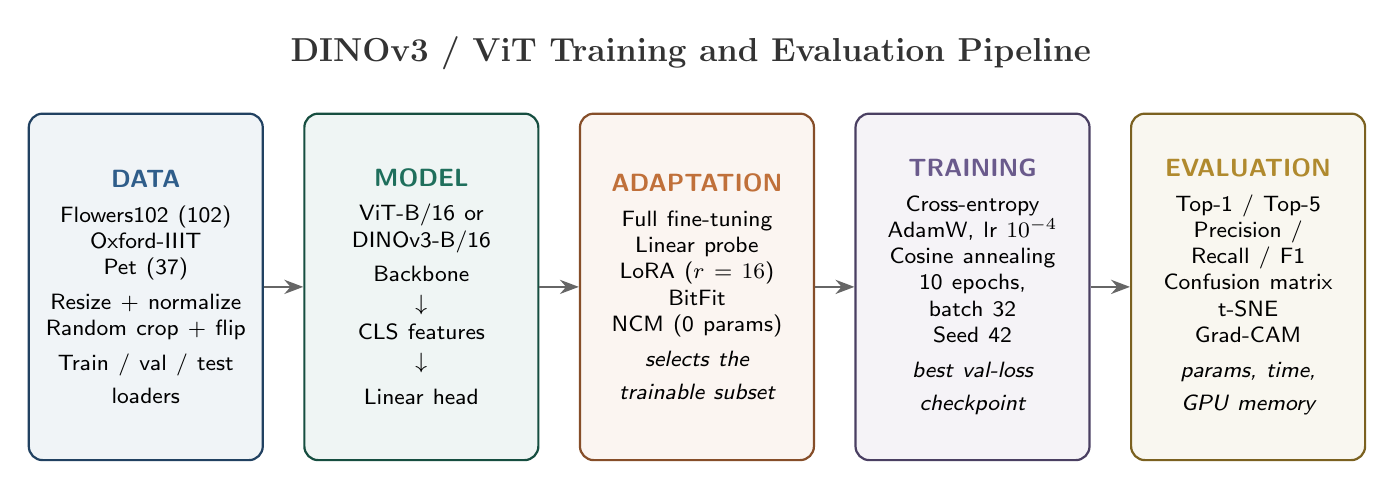
\begin{tikzpicture}[
    font=\sffamily,
    >=Stealth,
    node distance=0.5cm,
    card/.style={
        draw=#1!70!black,
        fill=#1!7,
        rounded corners=5pt,
        thick,
        align=center,
        text width=2.55cm,
        minimum height=4.4cm,
        inner sep=6pt
    },
    flow/.style={
        -{Stealth[length=2.4mm]},
        thick,
        draw=black!60
    }
]

% ------------------------------------------------------------------ %
% Five pipeline stages
% ------------------------------------------------------------------ %
\node[card=cData] (data) {
    {\textcolor{cData}{\bfseries\small DATA}}\\[3pt]
    {\footnotesize
    Flowers102 (102)\\
    Oxford-IIIT Pet (37)\\[3pt]
    Resize + normalize\\
    Random crop + flip\\[3pt]
    Train / val / test\\
    loaders}
};

\node[card=cModel, right=of data] (model) {
    {\textcolor{cModel}{\bfseries\small MODEL}}\\[3pt]
    {\footnotesize
    ViT-B/16 or\\
    DINOv3-B/16\\[3pt]
    Backbone\\[1pt]
    $\downarrow$\\[1pt]
    CLS features\\[1pt]
    $\downarrow$\\[1pt]
    Linear head}
};

\node[card=cAdapt, right=of model] (adapt) {
    {\textcolor{cAdapt}{\bfseries\small ADAPTATION}}\\[3pt]
    {\footnotesize
    Full fine-tuning\\
    Linear probe\\
    LoRA ($r=16$)\\
    BitFit\\
    NCM (0 params)\\[3pt]
    {\itshape selects the\\
    trainable subset}}
};

\node[card=cTrain, right=of adapt] (train) {
    {\textcolor{cTrain}{\bfseries\small TRAINING}}\\[3pt]
    {\footnotesize
    Cross-entropy\\
    AdamW, lr $10^{-4}$\\
    Cosine annealing\\
    10 epochs, batch 32\\
    Seed 42\\[3pt]
    {\itshape best val-loss\\
    checkpoint}}
};

\node[card=cEval, right=of train] (eval) {
    {\textcolor{cEval}{\bfseries\small EVALUATION}}\\[3pt]
    {\footnotesize
    Top-1 / Top-5\\
    Precision / Recall / F1\\
    Confusion matrix\\
    t-SNE\\
    Grad-CAM\\[3pt]
    {\itshape params, time,\\
    GPU memory}}
};

% ------------------------------------------------------------------ %
% Flow arrows
% ------------------------------------------------------------------ %
\draw[flow] (data.east) -- (model.west);
\draw[flow] (model.east) -- (adapt.west);
\draw[flow] (adapt.east) -- (train.west);
\draw[flow] (train.east) -- (eval.west);

% ------------------------------------------------------------------ %
% Title
% ------------------------------------------------------------------ %
\node[
    font=\large\bfseries,
    align=center,
    text=black!80
] at ($(data.north)!0.5!(eval.north)+(0,0.75)$) {
    DINOv3 / ViT Training and Evaluation Pipeline
};

\end{tikzpicture}

\end{document}
